
% !TeX spellcheck = pt_BR
% !TEX encoding = UTF-8 Unicode

\documentclass[b5paper]{article}

\usepackage[utf8]{inputenc}
\usepackage[T1]{fontenc}
\usepackage{lmodern}

% These are the default width and height for letterpaper
\usepackage[width=345pt,height=550pt,vmarginratio=1:1]{geometry}
\setlength{\footskip}{2em}

\usepackage{amsmath}
\usepackage{amsthm}
\usepackage[brazil]{babel}
\usepackage{graphicx}
\usepackage[hidelinks,colorlinks=true,urlcolor=blue,linkcolor=black,citecolor=black]{hyperref}
% \usepackage{nohyperref}

\usepackage[skins]{tcolorbox}

\tcbset{ bicolor, colback=lightgray!30!white, colbacklower=white, colframe=lightgray, boxsep=0pt,left=.5em,right=.5em,top=.5em,bottom=.5em, sharp corners, parbox=false }

\graphicspath{{figures/}{./}}

\hyphenpenalty 3000

\newcommand{\literal}[1]{\textsf{#1}}

% % Para retirar os literais:
% \renewcommand{\literal}[1]{lliitteerraallbe#1lliitteerraallen}
% \renewcommand{\LaTeX}{LaTeXx}
% \hyphenpenalty 10000
% \geometry{a4paper}
% \usepackage{newverbs}
% \newverbcommand{\myverb}{commannddbe}{commanndden}
% \newcommand{\rreff}[1]{rreff}
% % \verb| -> \myverb|
% % \ref{ -> \rreff{

\usepackage[notall]{embedall}
\embedfile{tutorial.zip}

\begin{document}

\title{\LaTeX\ Simplificado \footnotetext{\copyright 2019-\the\year\ Leonardo T. Rolla e Fábio L. B. Simas \href{https://creativecommons.org/licenses/by-sa/4.0/deed.pt_BR}{
\includegraphics[height=1em]{figures/by-sa.pdf}}}}
\author{Leonardo T. Rolla \and Fábio L. B. Simas}
\maketitle

\begin{abstract}
Este tutorial é uma introdução minimalista de \LaTeX, baseada em exemplos. O objetivo é suavizar a sua curva de aprendizagem.
\end{abstract}

\tableofcontents


\clearpage
\section{Começando com o pé direito}

Instale a versão completa de algum compilador de \LaTeX. Recomendamos
\href{http://tug.org/cgi-bin/mactex-download/MacTeX.pkg}
{\literal{\mbox{MacTeX}}}
para Mac, 
\href{http://tug.ctan.org/tex-archive/systems/texlive/Images/texlive.iso}
{\literal{TeX~Live}}
para Windows e
\literal{sudo apt install texlive-full}
para Ubuntu. Instalar a versão completa vai demorar muito e ocupar muito espaço, mas vai facilitar o seu aprendizado e evitar uma série de problemas no futuro.

Instale um editor integrado de \LaTeX.
Recomendamos o \literal{TeXstudio}.

Abra o \literal{TeXstudio}.
Vá em \literal{Options}, \literal{Configure TeXstudio}, \literal{General}, \literal{Language}, escolha \literal{pt\_BR} e clique \literal{OK}.
Agora vá em \literal{Opções}, \literal{Configurar}, \literal{Editor}, \literal{Modo de Recuo}, e escolha \literal{Ignorar Recuo}.

Crie um novo arquivo.
No editor, digite o seguinte:

\begin{tcolorbox}
\footnotesize
\begin{verbatim}
\documentclass{article}
\begin{document}
Meu primeiro texto em LaTeX :-)
\end{document}
\end{verbatim}
\end{tcolorbox}

Aperte \literal{F5} para compilar o arquivo.
(Se há uma advertência sobre mudança de atalhos padrão, ignore-a, marque ``não mostrar essa mensagem novamente'' e clique \literal{OK}).
Pronto!
O resultado esperado é o da Figura~\ref{fig:compilou}.

% Caso não tenha dado certo, o que é pouco provável, peça ajuda a um amigo.

\begin{figure}[b]
\centering
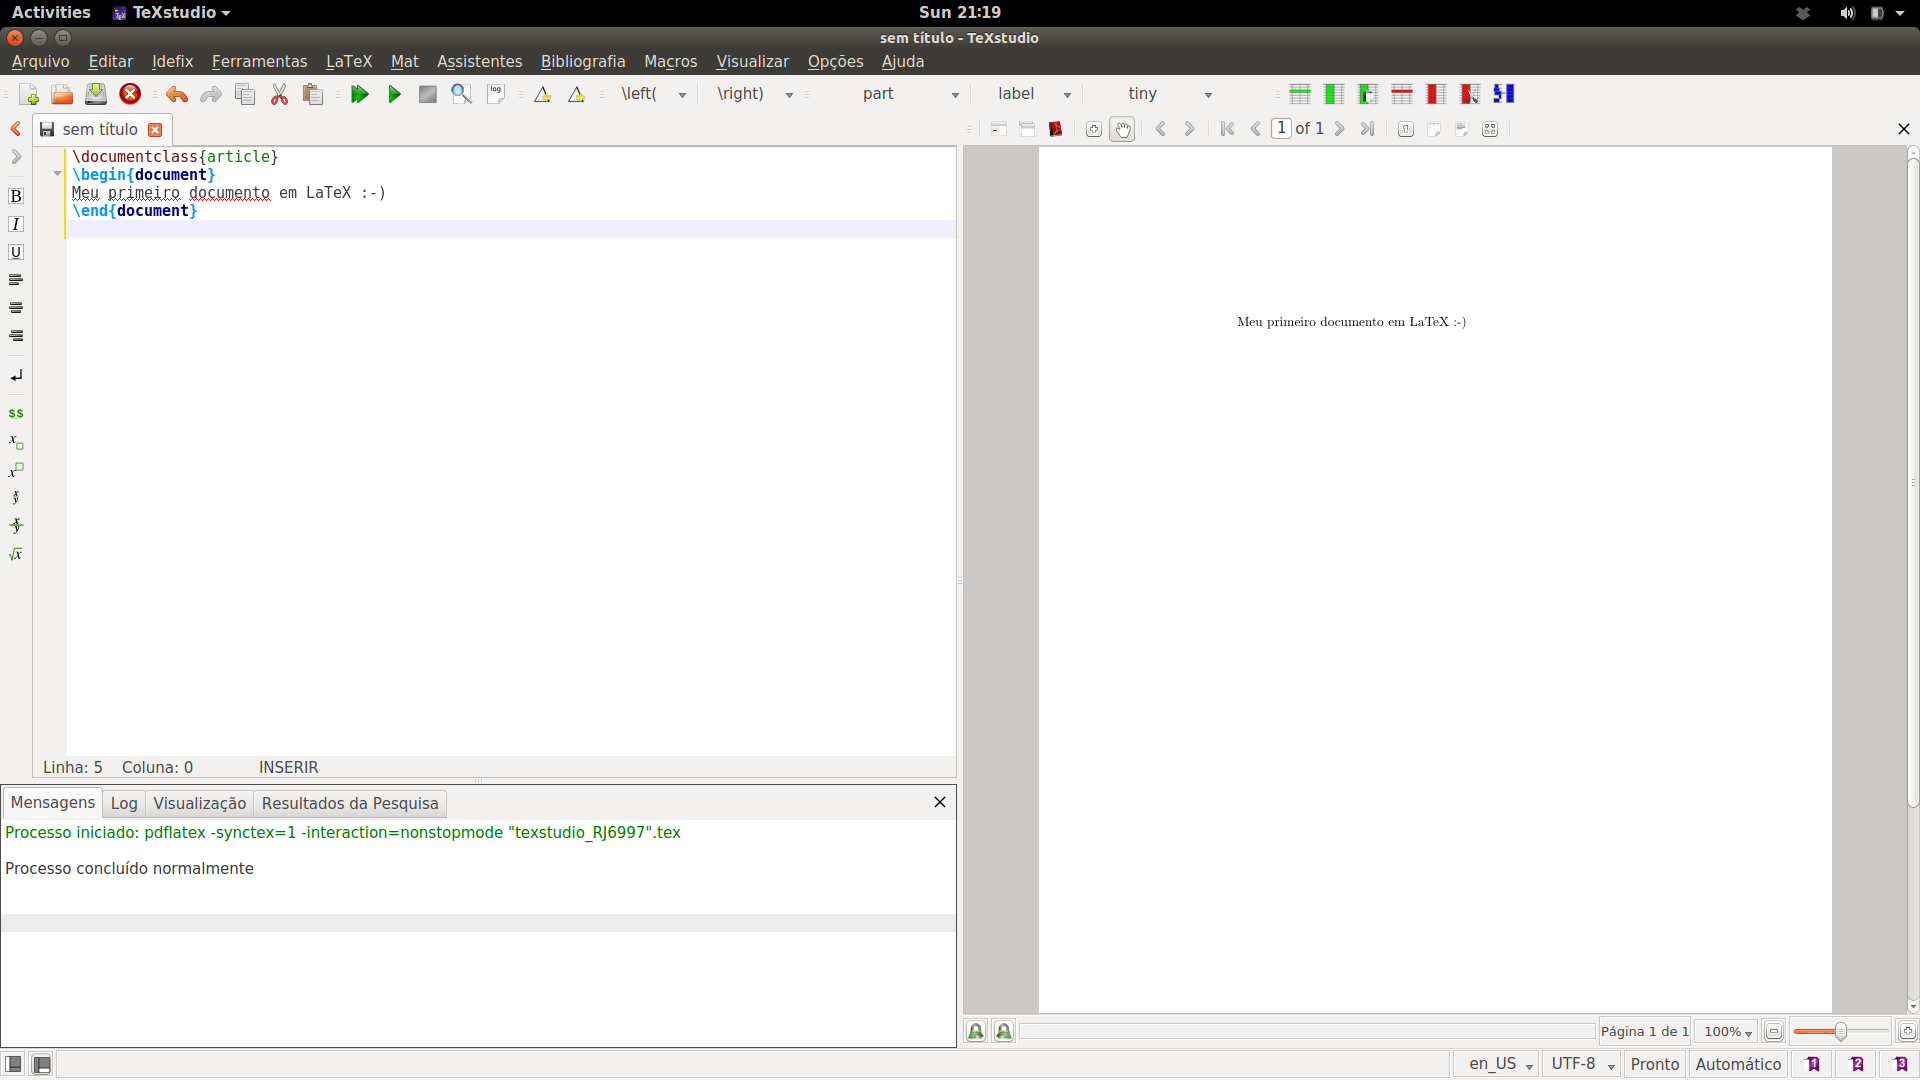
\includegraphics[width=.7\textwidth]{compile-pt.png}
\caption{Resultado esperado para o primeiro exemplo deste tutorial.}
\label{fig:compilou}
\end{figure}

Agora vamos testar se a instalação do \LaTeX\ está realmente completa.
Para isso, desconecte a Internet e compile o seguinte arquivo:

\begin{tcolorbox}
\footnotesize
\begin{verbatim}
\documentclass{article}
\usepackage{amsmath,amssymb,amsthm,bbm,booktabs,caption ,chngcntr,fontenc,
framed,enumitem,geometry,graphicx,hyperref,inputenc,lmodern,mathrsfs,microtype,
nameref,setspace,stmaryrd,tikz,ulem,vruler,wasysym,xcolor,xwatermark}
\begin{document}
Um documento que pede um monte de pacotes mas nao os usa.
\end{document}
\end{verbatim}
\end{tcolorbox}

Aperte \literal{F5} para compilar.
Antes de prosseguir, é importante assegurar-se de que o exemplo acima compila sem erros e sem mensagens de advertência.
% Caso contrário, no futuro você terá que lidar com erros sem saber qual a causa.

% Se der algum erro, peça ajuda a um amigo.

O próximo exemplo mostra como produzir textos que incluem letras acentuadas e contêm vários parágrafos.
Lembre-se de apertar \literal{F5} para compilar.

\begin{tcolorbox}
\footnotesize
\begin{verbatim}
\documentclass{article}
\usepackage[utf8]{inputenc}
\begin{document}
Este exemplo usa letras acentuadas como é, à, ã, ñ, ô, ç, etc.
Basta digitá-las normalmente e o compilador vai entender.

Outra novidade introduzida neste exemplo é a forma como podemos
criar novos
parágrafos em LaTeX: basta
deixar uma linha em branco.
\end{document}
\end{verbatim}
\tcblower
\indent
Este exemplo usa letras acentuadas como é, à, ã, ñ, ô, ç, etc. Basta
digitá-las normalmente e o compilador vai entender.

Outra novidade introduzida neste exemplo é a forma como podemos criar novos
parágrafos em LaTeX: basta deixar uma linha em branco.
\end{tcolorbox}

O \emph{preâmbulo} é tudo o que vem antes do {\footnotesize\verb|\begin{document}|}.
O comando {\footnotesize\verb|\documentclass{article}|} diz ao \LaTeX\ que este documento é um artigo e deve ser formatado como tal.
O comando {\footnotesize\verb|\usepackage[utf8]{inputenc}|} chama o pacote \literal{inputenc} com a opção \literal{utf8}, o que permite escrever usando letras com acento.

O \emph{corpo} do documento
é tudo o que está
entre os comandos {\footnotesize\verb|\begin{document}|} e {\footnotesize\verb|\end{document}|}.
A função destes comandos é justamente delimitar onde começa e termina o texto.

Agora você já pode escrever qualquer texto em \LaTeX.
Basta ir escrevendo e apertando \literal{F5} para compilar (fica muito mais fácil identificar erros se você compilar regularmente).
Você pode copiar material de qualquer outro editor, e ele vai compilar!
Lembre-se de deixar uma linha em branco entre os parágrafos.

Bem, na verdade, o \LaTeX\ vai compilar qualquer documento de texto que não contenha os dez símbolos:
``\& \% \$ \# \_ \{ \}
\textasciitilde\
\textasciicircum\
\textbackslash''.
Na próxima seção veremos como incluir esses e outros símbolos.


\clearpage
\section{Símbolos especiais}

O seguinte exemplo é auto-explicativo.

\begin{tcolorbox}
\footnotesize
\begin{verbatim}
\documentclass{article}
\usepackage[utf8]{inputenc}
\usepackage[T1]{fontenc}
\usepackage{lmodern}
\begin{document}
O LaTeX usa os símbolos \& \$ \# \_ \{ \} \%
\textasciitilde \ \textasciicircum \ \textbackslash \ para outros
fins. Por isso, incluir
esses símbolos no texto requer o uso de comandos específicos.

Outros símbolos especiais são: \LaTeX,
\copyright, \S, dentre vários outros que você vai aprender gradualmente.

% Veja que esta linha não vai produzir texto.

A forma correta de inserir aspas `simples' e ``duplas'' é esta.
\end{document}
\end{verbatim}
\tcblower
\indent
O LaTeX usa os símbolos \& \$ \# \_ \{ \} \%
\textasciitilde \ \textasciicircum \ \textbackslash \ para outros
fins. Por isso, incluir
esses símbolos no texto requer o uso de comandos específicos.

Outros símbolos especiais são: \LaTeX,
\copyright, \S, dentre vários outros que você vai aprender gradualmente.

A forma correta de inserir aspas `simples' e ``duplas'' é esta.
\end{tcolorbox}

% Lembre-se que nossos exemplos mostram apenas o corpo do documento, omitindo {\footnotesize\verb|\begin{document}|}, {\footnotesize\verb|\end{document}|} e o preâmbulo!
% 
% \medskip

Os símbolos especiais têm as seguintes finalidades:
\begin{center}
\begin{tabular}{cp{.8\textwidth}}
\texttt{\small \textbackslash} & início de comandos.
\\
\texttt{\small \{ \}} & delimitam um bloco de texto ou símbolos.
\\
\texttt{\small \textasciitilde} & insere um espaço que não permite quebra de linha.
\\
\texttt{\small \$} &marca o início e o fim de expressões matemáticas.
\\
\texttt{\small \textasciicircum \ \_} &superíndice ($a^n$) e subíndice ($a_n$) em expressões matemáticas.
\\
\texttt{\small \%} &diz ao compilador para ignorar o resto da linha.
\\
\texttt{\small \&} &alinhamento em tabelas, equações, matrizes, etc.
\\
\texttt{\small \#} &usado para criar macros (avançado).
\end{tabular}
\end{center}

Uma barra {\footnotesize\verb|\|} sozinha cria \ um espaço \ extra. Duas barras, separadas por um espaço, criam \ \ dois espaços \ \ extras.
Repare que, no início do exemplo, os comandos {\footnotesize\verb|\textasciitilde|}, {\footnotesize\verb|\textasciicircum|} e {\footnotesize\verb|\textbackslash|} requerem uma barra, assim o símbolo sai \textasciitilde\ separado do texto que o sucede ao invés de \textasciitilde colado.

Duas barras juntas {\footnotesize\verb|\\|} causam uma quebra
\\
no texto, e servem para delimitar uma linha em equações, matrizes e tabelas.

\medskip

O pacote \literal{fontenc} com opção \literal{T1} especifica a codificação dos símbolos no \literal{pdf} que será gerado.
O pacote \literal{lmodern} inclui uma fonte idêntica à fonte padrão do \LaTeX, porém com alguns caracteres a mais e outros com tipografia melhorada.

\clearpage
\section{Formatação básica de texto}
\label{sec-formatacao}

O exemplo a seguir ilustra algumas das formatações mais frequentes.

\begin{tcolorbox}
\footnotesize
\begin{verbatim}
\documentclass{article}
\usepackage[utf8]{inputenc}
\begin{document}
O tamanho da fonte pode ser alterado para {\Huge super}, {\huge enorme},
{\Large muito grande}, {\large grande}, {\small pequeno} e {\tiny minúsculo}.

Para obter texto centralizado e espaçado,

\begin{center}
Fazemos assim!
\end{center}

Assim escrevemos em \textbf{negrito}, \textit{itálico} e \emph{enfatizado}.
\end{document}
\end{verbatim}
\tcblower
\indent
O tamanho da fonte pode ser alterado para {\Huge super}, {\huge enorme},
{\Large muito grande}, {\large grande}, {\small pequeno} e {\tiny minúsculo}.

Para obter texto centralizado e espaçado,

\begin{center}
Fazemos assim!
\end{center}

Também podemos escrever em \textbf{negrito}, \textit{itálico} e \emph{enfatizado}.
\end{tcolorbox}

O \LaTeX\ privilegia \emph{conteúdo} e \emph{semântica} sobre \emph{formatação direta}.
Isso quer dizer que o Autor de um texto deve estar focado no conteúdo do texto e não na apresentação.
A formatação será decida pelo Editor, através de escolha uma classe ({\footnotesize\verb|\documentclass|}) e do uso de pacotes ({\footnotesize\verb|\usepackage|}).

O comando {\footnotesize\verb|\emph|} acima é um comando \emph{semântico}, em que o Autor expressa sua \emph{intenção} de que essa parte do texto seja enfatizada.
O fato de que esse comando resulta em texto itálico é casual.
Em outros contextos, a forma de enfatizar pode ser algo diferente do itálico (ou até mesmo a ausência deste).

O comando 
{\footnotesize\verb|\begin{center}|}
também é, certa forma, um comando semântico.
Ele expressa a intenção do Autor que essa parte do texto deve vir destacada e separada do resto, sem especificar qual a distância que deve separá-los.

Nesse espírito, dentre os comandos utilizados acima recomendamos apenas o uso desses dois.
Sugerimos evitar ao máximo o uso dos outros recursos aqui ilustrados.
Ficar pensando em formatação vai contra a filosofia do \LaTeX.


\clearpage
\section{Seções e referências internas}
\label{sec-estrutura}

\begin{tcolorbox}
\footnotesize
\begin{verbatim}
\documentclass{article}
\usepackage[utf8]{inputenc}
\begin{document}
\section{Título da seção}
Texto introdutório desta seção.
\subsection{Título da subseção}
Texto da subseção.
\subsection{Título de outra subseção}
Também é possível criar seções ou subseções sem numeração usando *.
\section{Título}
\label{sec:rotulo-escolhido}
Aqui uma outra seção.
\section*{Título da seção sem numeração}
Ao contrário da Seção~\ref{sec:rotulo-escolhido} acima, esta não é numerada.
\end{document}
\end{verbatim}
\newcounter{ondeestava}
\setcounter{ondeestava}{\thesection}
\setcounter{section}{0}
\tcblower
\section*{1 \ \ Título da seção}
Texto introdutório desta seção.
\subsection*{1.1 \ \ Título da subseção}
Texto da subseção.
\subsection*{1.2 \ \ Título de outra subseção}
Também é possível criar seções ou subseções sem numeração usando *.
\section*{2 \ \ Título}
Aqui uma outra seção.
\section*{Título da seção sem numeração}
Ao contrário da Seção~2 acima, esta não é numerada.
\end{tcolorbox}
\setcounter{section}{\theondeestava}

Use um \emph{rótulo} (\literal{label}) para identificar uma seção quando quiser fazer posterior \emph{referência} (\literal{ref}). 
Veja que o exemplo acima não contém o número 2, ele foi gerado pelo \LaTeX.
Se o número da seção mudar (por exemplo, porque uma seção foi acrescentada ou removida antes dessa, ou porque o estilo de numeração de seções foi alterado), a referência será atualizada automaticamente.
O mesmo serve para referenciar capítulos, subseções, itens em uma lista numerada, figuras
e tabelas.

O formato dos títulos de seções e subseções foi determinado pela escolha de estilo \emph{artigo}, na primeira linha do preâmbulo.
Outros estilo de documento resultarão em outro formato, mas o Autor não deve se preocupar com isso.


\clearpage
\section{Incluir bibliografia}
\label{sec-bibliografia}

No exemplo a seguir há comentários no código, eles são sempre iniciados pelo símbolo {\footnotesize\verb|%|}, que indica ao compilador que ignore o restante da linha.

\begin{tcolorbox}
\footnotesize
\begin{verbatim}
\documentclass{article}
\usepackage[utf8]{inputenc}
\usepackage[brazil]{babel} % seleção de idioma
\begin{document}
Neste exemplo vamos citar os livros~\cite{Carmo} e~\cite{James}.
\begin{thebibliography}{11}
\bibitem{Carmo}
M.~P. do~Carmo. \emph{Geometria Riemanniana}. IMPA, 1988.
\bibitem{James}
B.~R. James. \emph{Probabilidade: Um Curso em Nível
Intermediário,} 2a.~edição. IMPA, Rio de Janeiro, 2002.
\end{thebibliography}
\end{document}
\end{verbatim}
\tcblower
\indent
Neste exemplo vamos citar os livros~\cite{Carmo} e~\cite{James}.
\begin{thebibliography}{11}
\bibitem{Carmo}
M.~P. do~Carmo. \emph{Geometria Riemanniana}. IMPA, 1988.
\bibitem{James}
B.~R. James. \emph{Probabilidade: Um Curso em Nível Intermediário,} 2a.~edição.
IMPA, Rio de Janeiro, 2002.
\end{thebibliography}
\end{tcolorbox}

Esta é uma forma simples e rudimentar de se inserir referências. Usuários experientes utilizam \literal{BibTeX}, que não vamos abordar neste tutorial.

O pacote \literal{babel} com a opção \literal{brazil} no preâmbulo faz com que o título ``Referências'' apareça em português.
De fato, ele faz com que muitos outros pacotes gerem texto em português, além de hifenizar palavras do seu documento segundo este idioma.


\clearpage
\section{Formatação básica de página}

% O tamanho padrão depende da instalação.
% Com pdfLaTeX não adianta só por a opção em documentclass

O tamanho do papel pode ser escolhido entre \literal{a4paper}, \literal{a5paper}, \literal{b5paper}, \literal{letterpaper}, ou \literal{legalpaper}, alterando-se a primeira linha do preâmbulo.

O exemplo abaixo gera um documento com tamanho de página Legal.
O pacote \literal{Geometry} com opção \literal{pass} faz o compilador passar a informação de tamanho de página ao arquivo \literal{pdf} sem no entanto fazer nenhuma outra alteração no documento.
\begin{tcolorbox}
\footnotesize
\begin{verbatim}
\documentclass[legalpaper]{article}
\usepackage[pass]{geometry}
\end{verbatim}
\end{tcolorbox}
% Sem o \usepackage[pass]{geometry}, o pdflatex não gera a página com o tamanho do documentclass!

No exemplo a seguir, o papel é A4 e nas páginas ímpares temos margem esquerda=30mm, direita=21mm, superior=22mm e inferior=23mm.
Devido à opção \literal{twoside}, intercambiam-se as margens direita e esquerda nas páginas pares, o que é muito útil caso o documento seja impresso em frente-e-verso.

\begin{tcolorbox}
\footnotesize
\begin{verbatim}
\documentclass[twoside,a4paper]{article}
\usepackage[left=30mm,right=21mm,top=22mm,bottom=23mm]{geometry}
\end{verbatim}
\end{tcolorbox}

O tamanho padrão da fonte é \literal{10pt}.
Para mudar o tamanho para \literal{11pt} ou \literal{12pt}, declare isso na primeira linha como no exemplo a seguir.
Se você tem um bom motivo para produzir um documento inteiro baseado em outro tamanho de fonte, vai precisar de pacotes adicionais.

\begin{tcolorbox}
\footnotesize
\begin{verbatim}
\documentclass[oneside,letterpaper,11pt]{article}
\usepackage[left=30mm,right=21mm,top=22mm,bottom=23mm]{geometry}
\end{verbatim}
\end{tcolorbox}
\vspace{-.5em}
\noindent
Neste exemplo, o papel é Carta e as páginas ímpares e pares são iguais.

\medskip

O exemplo a seguir altera o espaçamento entre as linhas para duplo e retira o recuo dos parágrafos.
Ele também aumenta o espaçamento entre dois parágrafos, que passa a ter, além do espaço normal entre linhas, mais 75\% da altura de uma linha do texto.

\begin{tcolorbox}
\footnotesize
\begin{verbatim}
\documentclass{article}
\usepackage{setspace} % pacote necessário para usar setstretch
\setstretch{2.0} % espaçamento duplo entre linhas
\setlength{\parindent}{0.0em} % parágrafo sem recuo
\setlength{\parskip}{0.75em} % espaçamento extra entre parágrafos
\end{verbatim}
\end{tcolorbox}


\clearpage
\section{Expressões matemáticas}
\label{sec-matematica}

\begin{tcolorbox}
\footnotesize
\begin{verbatim}
\documentclass{article}
\usepackage[utf8]{inputenc}
\usepackage{amsmath} % Provê o ambiente align
\begin{document}
As raízes da equação $ax^2 + bx + c = 0$ com a variável $x$ são
\[
x = \frac{ -b \pm \sqrt{b^2-4ac} }{ 2a }.
\]
Temos somatórios e frações como em
\begin{equation}
\label{eq:serie}
\sum_{n=0}^{\infty} \frac{1}{3^n} = \frac{1}{1 - \frac{1}{3}} = \frac{3}{2}.
\end{equation}
Também temos equações alinhadas, integrais e escolha de tamanho:
\begin{align}
\int_1^\infty e^{-x^2} \mathrm{d} x & \leq \int_1^\infty e^{-x}
\mathrm{d} x \label{eq:integral}
\\
& = \lim_{t\to\infty} -e^{-x} \, \Big]_1^t \nonumber
\\
& = 1. \nonumber
\end{align}
Em~(\ref{eq:serie}) usamos a fórmula da série geométrica e
em~(\ref{eq:integral}) usamos a comparação dos integrandos.
\end{document}
\end{verbatim}
\tcblower
\indent
As raízes da equação $ax^2 + bx + c = 0$ com a variável $x$ são
\[ x = \frac{ -b \pm \sqrt{b^2-4ac} }{ 2a }. \]
Temos somatórios e frações como em
\begin{equation}\label{eq:serie}
\sum_{n=0}^{\infty} \frac{1}{3^n} = \frac{1}{1 - \frac{1}{3}} = \frac{3}{2}.
\end{equation}
Também temos equações alinhadas, integrais e escolha de tamanho:
\begin{align}
\int_1^\infty e^{-x^2} \mathrm{d} x & \leq \int_1^\infty e^{-x} \mathrm{d} x
\label{eq:integral} \\
& = \lim_{t\to\infty} -e^{-x} \, \Big]_1^t \nonumber \\
& = 1. \nonumber
\end{align}
Em~(\ref{eq:serie}) usamos a fórmula da série geométrica e
em~(\ref{eq:integral}) usamos a comparação dos integrandos.
\end{tcolorbox}

Com superíndice {\footnotesize\verb|^|} que usamos para escrever $x^2$ e o
subíndice {\footnotesize\verb|_|} que usamos para escrever $x_1$, também podemos especificar
limites de somatórios e integrais.


\clearpage
\section{Ambientes tipo teorema}

\begin{tcolorbox}
\footnotesize
\begin{verbatim}
\documentclass{article}
\usepackage{amsthm}
\usepackage[utf8]{inputenc}

\theoremstyle{plain} % Estilo de ambiente padrão
\newtheorem{teorema}{Teorema} % Criando ambiente teorema

\theoremstyle{definition} % Estilo de ambiente sem itálico
\newtheorem{definicao}{Definição} % Criando ambiente definicao
\newtheorem{exercicio}{Exercício} % Criando ambiente exercicio
\newtheorem*{solucao}{Solução} % Criando ambiente solucao

\theoremstyle{remark} % Estilo com título em itálico
\newtheorem{comentario}{Comentário} % Criando ambiente comentario

\begin{document}
\begin{definicao}
Definimos o \emph{diâmetro} de $S$ como
$\mathrm{diam} S = \sup\limits_{x,y \in S} d(x,y)$.
\end{definicao}
\begin{teorema}
Se $A \subseteq B$ então $\mathrm{diam} A \leq \mathrm{diam} B$.
\end{teorema}
\begin{exercicio}
Se $A \cap B \ne \emptyset$, mostre que $\mathrm{diam} (A \cup B) \leq
\mathrm{diam} A + \mathrm{diam} B$.
\end{exercicio}
\begin{solucao}
Aqui você pode completar com sua própria solução.
\end{solucao}
\begin{comentario}
Diâmetro é um conceito muito útil.
\end{comentario}
\end{document}
\end{verbatim}
\tcblower
\theoremstyle{plain}
\newtheorem{teorema}{Teorema}
\theoremstyle{definition}
\newtheorem{definicao}{Definição}
\newtheorem{exercicio}{Exercício}
\newtheorem*{solucao}{Solução}
\theoremstyle{remark}
\newtheorem{comentario}{Comentário}
\begin{definicao}
Definimos o \emph{diâmetro} de $S$ como
$\mathrm{diam} S = \sup\limits_{x,y \in S} d(x,y)$.
\end{definicao}
\begin{teorema}
Se $A \subseteq B$ então $\mathrm{diam} A \leq \mathrm{diam} B$.
\end{teorema}
\begin{exercicio}
Se $A \cap B \ne \emptyset$, mostre que $\mathrm{diam} (A \cup B) \leq
\mathrm{diam} A + \mathrm{diam} B$.
\end{exercicio}
\begin{solucao}
Aqui você pode completar com sua própria solução.
\end{solucao}
\begin{comentario}
Diâmetro é um conceito muito útil.
\end{comentario}
\end{tcolorbox}

Neste exemplo há três estilos de ambientes predefinidos: o estilo padrão \literal{plain}, usado para Teorema, e os estilos \literal{definition} e \literal{remark}. Repare que o ambiente \literal{solucao} não possui numeração, devido ao \literal{*} no preâmbulo. Nomes de ambientes não podem ser acentuados.


\clearpage
\section{Incluir figuras}

\begin{tcolorbox}
\footnotesize
\begin{verbatim}
\documentclass{article}
\usepackage[utf8]{inputenc}
\usepackage[brazil]{babel} % faz com que "Figura" apareça em português
\usepackage{graphicx} % fornece o comando \includegraphics
\begin{document}
A Figura~\ref{fig:seta} contém duas versões da mesma imagem, uma
com a altura de 4 linhas de texto e outra com 25\% da largura de um parágrafo.
\begin{figure}[bp]
\centering

\includegraphics[height=4em]{nick-fewings.jpg}

\includegraphics[width=0.25\textwidth]{nick-fewings.jpg}
\caption{Imagem de Nick Fewings, disponível no Unsplash.}
\label{fig:seta}
\end{figure}

Veja que a Figura~\ref{fig:seta} foi inserida entre este parágrafo e o
anterior, mas no documento final não sabemos exatamente onde ela vai aparecer.
\end{document}
\end{verbatim}
\tcblower
\indent
A Figura~\ref{fig:seta} contém duas versões da mesma imagem, uma
com a altura de 4 linhas de texto e outra com 25\% da largura de um parágrafo.

Veja que a Figura~\ref{fig:seta} foi inserida entre este parágrafo e o
anterior, mas no documento final não sabemos exatamente onde ela vai aparecer.
\end{tcolorbox}

\begin{figure}[bp]
\centering

\includegraphics[height=4em]{nick-fewings.jpg}

\includegraphics[width=0.25\textwidth]{nick-fewings.jpg}
\caption{Imagem de Nick Fewings, disponível no Unsplash.}
\label{fig:seta}
\end{figure}

% As opções mais comuns são {\footnotesize\verb|scale|}, {\footnotesize\verb|width|} e {\footnotesize\verb|height|}, todos redimensionam a figura especificando respectivamente um fator de escala, a largura e a altura da figura.
% Eu nunca vi utilidade no scale. Uso em menos de 1% dos casos.

% O arquivo pode ser incluído com o comando {\footnotesize\verb|\includegraphics|}, fornecido pelo pacote \literal{graphicx}, e que deve aparecer entre {\footnotesize\verb|\begin{figure}|} e {\footnotesize\verb|\end{figure}|}.

O ambiente \literal{figure} é um \emph{ambiente flutuante}.
Sua posição será decidida pelo compilador em função de critérios estéticos: não deixar muito espaço em branco, não deixar uma ou duas linhas isoladas do resto do texto, etc.

Ao usar \LaTeX, o Autor não deve pensar na figura como tendo uma localização exata.
No princípio, temos a tendência a esperar que a figura apareça ``bem aqui'', mas depois aprendemos a apreciar as vantagens de tê-la, por exemplo, no pé da página.
A forma apropriada de conectar o texto com a figura é fazendo-se referência explícita, como ``Figura~\ref{fig:seta}''.
Também fizemos isso com a Figura~\ref{fig:compilou}.

O parâmetro \literal{[bp]} no exemplo acima diz ao compilador para tentar acomodar a figura em algum \emph{pé de página} (\literal{b}) ou, se não ficar muito bom, em uma \emph{página separada} (\literal{p}).
Outras possibilidades são \literal{h} para \emph{aqui} e \literal{t} para \emph{topo de página}.

O comando {\footnotesize\verb|\caption|} cria uma legenda e dá um número à figura.
Após a legenda, pode-se usar o comando {\footnotesize\verb|\label|} para associar o número a um rótulo.

Você pode incluir imagens em formato \literal{pdf}, \literal{png} ou \literal{jpg}, basta salvá-las na mesma pasta em que se encontra o arquivo \literal{tex}.


\clearpage
\section{Incluir tabelas}

Veremos um exemplo rudimentar de tabela sem alinhamento vertical nem células múltiplas, e com alinhamento horizontal uniforme em cada coluna.

O alinhamento horizontal de cada coluna pode ser centralizado, à esquerda, à direita, ou justificado (\literal{clrp}).
Neste último, a largura deve ser especificada.

% Nos três primeiros casos, a largura da coluna será determinada pelo conteúdo de suas células.
% {\footnotesize\verb|p{"largura"}|}.

% Para inserir tabelas, deve ser indicada a posição desejada do texto em cada uma das colunas. As opções padrão são: 

%Nos três primeiros casos, não há quebra de linha nas células.
% O ambiente \literal{table} é usado para numerar e possibilitar o inserção de legenda.
%Veja alguns exemplos.

\begin{tcolorbox}
\footnotesize
\begin{verbatim}
\documentclass{article}
\usepackage[utf8]{inputenc}
\usepackage[brazil]{babel} % faz com que "Tabela" apareça em português
\begin{document}
A Tabela~\ref{tab:exemplo} tem todos os tipos de alinhamento, incluindo uma
coluna justificada que ocupa 33\% da largura de um parágrafo.
\begin{table}[bp]
\centering
\begin{tabular}{|| c r  l | p{.33\textwidth} ||}
\hline \hline
x & y & valor total & Obs. \\
\hline \hline
1 & 2 & 793 & observação curta \\
\hline
411,00 & 2 & 7 & observação longa demais para uma linha \\
\hline
4 & 742 & 43 & \\
c & d & e & j \\
\hline \hline
\end{tabular}
\caption{Coleção de números e observações sem sentido.}
\label{tab:exemplo}
\end{table}

Como no caso das figuras, inserimos a Tabela~\ref{tab:exemplo} entre este
parágrafo e o anterior, mas não sabemos onde ela vai aparecer.
\end{document}
\end{verbatim}
\tcblower
\indent
A Tabela~\ref{tab:exemplo} tem todos os tipos de alinhamento, incluindo uma coluna justificada que ocupa 33\% da largura de um parágrafo.

Como no caso das figuras, inserimos a Tabela~\ref{tab:exemplo} entre este
parágrafo e o anterior, mas não sabemos onde ela vai aparecer.
\end{tcolorbox}

\begin{table}[bp]
\centering
\begin{tabular}{|| c r  l | p{.33\textwidth} ||}
\hline \hline
x & y & valor total & Obs. \\
\hline \hline
1 & 2 & 793 & observação curta \\
\hline
411,00 & 2 & 7 & observação longa demais para uma linha \\
\hline
4 & 742 & 43 & \\
c & d & e & j \\
\hline \hline
\end{tabular}
\caption{Coleção de números e observações sem sentido.}
\label{tab:exemplo}
\end{table}

Repare que \literal{table} também é um \emph{ambiente flutuante.}
Não sabemos onde a Tabela~\ref{tab:exemplo} vai aparecer, para conectá-la ao texto fazemos referência explícita.

% \clearpage
% \section{Incluir listas}
% 
% x


\clearpage
\section{Bons e maus hábitos}

É muito comum que um amigo ou colega bem-intencionado nos forneça um arquivo enorme, cheio de pacotes e comandos e que não temos a menor ideia de para quê servem.
Recomendamos criar um novo preâmbulo contendo apenas o necessário para cada documento, e não usar esses arquivos enormes.

\medskip

Antes de {\footnotesize\verb|\ref|} e {\footnotesize\verb|\cite|}, use {\footnotesize\verb|~|} ao invés de espaço.
Assim, a referência ``Seção\linebreak[4] 2'' nunca vai aparecer quebrada em linhas diferentes como neste parágrafo.

\medskip

Os comandos abaixo são obsoletos, susceptíveis de erro, ou incorretos:

\begin{tcolorbox}
\footnotesize
\begin{verbatim}
[utf8x], {\it texto}, {\bf texto}, $$ x=y $$, {eqnarray}, \let & \def
\end{verbatim}
\end{tcolorbox}

As alternativas corretas são, respectivamente:

\begin{tcolorbox}
\footnotesize
\begin{verbatim}
[utf8], \emph{texto}, \textbf{texto}, \[ x=y \], {align}, \newcommand
\end{verbatim}
\end{tcolorbox}

Os seguintes comandos também não devem ser usados:

\begin{tcolorbox}
\footnotesize
\begin{verbatim}
\baselinestretch, \def, \sloppy, \centerline, doublespace
\end{verbatim}
\end{tcolorbox}

\medskip

Sempre é bom usar os seguintes pacotes:

\begin{tcolorbox}
\footnotesize
\begin{verbatim}
\usepackage[utf8]{inputenc}
\usepackage[T1]{fontenc}
\usepackage{lmodern}
\end{verbatim}
\end{tcolorbox}

O pacote \literal{inputenc} faz com que o compilador entenda letras acentuadas, entre outros símbolos.
O pacote \literal{fontenc} faz gerar um \literal{pdf} em que ``á'' seja um único símbolo ao invés da justaposição do símbolo ``\'{}'' com o símbolo ``a'' logo abaixo.
Isso é muito prático para que o leitor possa pesquisar palavras ou copiar texto do documento.
Ao utilizar-se o pacote \literal{fontenc}, é necessário utilizar o pacote \literal{lmodern} para que a fonte seja incluída corretamente no arquivo \literal{pdf}.
Caso não haja letras acentuadas no documento, podem-se omitir esses três pacotes.


\clearpage
\section{Comentários finais}

\LaTeX\ é uma ferramenta que produz textos de altíssima qualidade tipográfica.
Em comparação com os editores de texto mais populares,
\LaTeX\
introduz
um paradigma que privilegia \emph{conteúdo} e \emph{semântica} ao invés da \emph{formatação direta}.
Este tutorial resume de forma minimalista seus aspectos mais básicos.

Começamos pelo mais essencial: criar textos básicos com parágrafos, bem como inserir os símbolos que foram apropriados pelo \LaTeX\ para seu uso interno.
Depois descrevemos algumas das formas mais básicas de formatação direta, apesar de desencorajar o seu uso.
Também explicamos como dar estrutura ao texto e incluir bibliografia.
Em seguida, demos exemplos básicos de como controlar a formatação de página e espaçamento, incluir expressões matemáticas e ambientes de texto destacado.
Finalmente,
vimos como inserir figuras e tabelas, a noção de ambientes flutuantes, e como eles devem ser referenciados no corpo do texto.
Terminamos mencionando alguns maus hábitos que você deve evitar.

Você eventualmente necessitará procurar material mais avançado quando quiser gerar outros tipos de documentos além de artigos, usar outros recursos de formatação, etc.
Ao produzir documentos maiores e com várias referências bibliográficas, você também deverá aprender o uso de \literal{BibTeX}.

Nosso público-alvo principal são pessoas que sabem apreciar as vantagens do \LaTeX\ mas ainda não sabem usá-lo.
Não pretendemos contudo que este seja o material mais indicado para qualquer pessoa nessa situação.
Tampouco pretendemos que este tutorial substitua manuais já existentes.
Nossa proposta é que as pessoas comecem a produzir documentos de qualidade mesmo tendo o mínimo de conhecimento técnico, e que possam ir aprendendo seus aspectos mais sofisticados apenas à medida em que efetivamente os necessitem.


\end{document}
